\documentclass{book}[12pt, a4paper, twoside] % Tipo de documento y tamaño de letra.

%%%%%%%%% Preambulo %%%%%%%%%%%%%%%%

% Para modificar los margenes. 
\usepackage{geometry}
\geometry{
    a4paper,
    left=20mm,
    top=20mm,
    right=20mm,
    bottom=20mm,
}

\usepackage[T1]{fontenc}
\usepackage{tocloft}
\usepackage{titlesec}
\setlength{\parskip}{1em} % Ajusta el valor según tus necesidades

\titleformat{\section}[hang]{\normalfont\bfseries}{\thesection}{0.5em}{}
\titleformat{\subsection}[hang]{\normalfont\bfseries}{\thesubsection}{0.5em}{}
\titleformat{\subsubsection}[hang]{\normalfont\bfseries}{\thesubsubsection}{0.5em}{}



% Para la bibliografia.
\usepackage[square,numbers]{natbib}
\usepackage{bibentry}
\nobibliography*

% Recursos personales.

\newcommand\asignatura{
Minería de Datos
}

\newcommand\nombrepec{
\vspace{0.25cm}
Proyecto de minería de datos

}

\newcommand\numeropec{
2
}

% \newcommand{\pec}{PEC}
\newcommand{\PRA}{PRA}

\newcommand\autor{
Álvaro Monforte Marín
}

\newcommand\tipopuntuacion{
% \%
% points
% puntos
p
}



%%%%%%%%%%%%%%%%%%%%%%%%%%%%%%%%%%%%%%%%%%%%%%%%%%%%%%%%%%%%%%%%%%%%%%%%%%%%%%%
% Funciones propias:
%%%%%%%%%%%%%%%%%%%%%%%%%%%%%%%%%%%%%%%%%%%%%%%%%%%%%%%%%%%%%%%%%%%%%%%%%%%%%%%

% Para realizar ejercicios
\newcommand{\ejercicio}[3]{
\ifthenelse{\equal{#1}{true}}{\newpage}{}
\section{Ejercicio #2 \normalsize \textbf{$[#3 \tipopuntuacion]$}}
}

% % Para realizar practicas
% \newcommand{\tematica}[4]{
% \ifthenelse{\equal{#1}{true}}{\newpage}{}
% \section{#2 \textbf{$[#3 \text{\tipopuntuacion}]$}}
% \textbf{#4}
% \vspace{0.15cm}
% % \subsubsection{Respuesta/as al #2}
% }

% \newcommand{\subtematica}[4]{
% \ifthenelse{\equal{#1}{true}}{\newpage}{}
% \subsection{#2 \textbf{$[#3 \text{\tipopuntuacion}]$}}
% \textbf{#4}
% \vspace{0.15cm}
% % \subsubsection{Respuesta/as al #2}
% }


% Para introducir imagenes
% (ejemplo: \insertimage{nombre_de_la_imagen}{ancho_de_la_imagen}{leyenda_de_la_imagen})

\usepackage{graphicx}
\usepackage{float}

\newcommand{\imagen}[3]{
\begin{figure}[H]
\centering
\includegraphics[scale=#2]{#1}
\caption[#3]{#3}
\label{fig:#1}
\end{figure}
}


%%%%%%%%%%%%%%%%%%%%%%%%%%%%%%%%%%%%%%%%%%%%%%%%%%%%%%%%%%%%%%%%%%%%%%%%%%%%%%%%%%%%%%
\newcommand{\documento}[2]{\href{#1}{#2}}
%%%%%%%%%%%%%%%%%%%%%%%%%%%%%%%%%%%%%%%%%%%%%%%%%%%%%%%%%%%%%%%%%%%%%%%%%%%%%%%%%%%%%%


%%%%%%%%%%%%%%%%%%% VARIABLES GLOBALES DEFINIDAS
\newcommand{\mongodb}{\href{https://www.mongodb.com/}{MongoDB} }


% EDICION
\newcommand{\propertyofauthor}[1]{Produced and edited by the author of this document using #1.}
\newcommand{\propiedadautor}[1]{Producido y editado por el autor de este documento usando #1.}
\newcommand{\propiedaddeautor}[1]{Producido y editado por el autor de este documento usando #1.}
\newcommand{\latex}{\LaTeX}

%%%%%%%%%%%%%%%%%%%%%%%%%%%%%%%%%%%%%%%%%%%%%%%%%%%%%%%%%%%%%%%%%%%%%%%%%%%%


%%%%%%%%%%%%%%%%%%%%%%%%%%%%%%%%%%%%%%%%%%%%%%%%%%%%%%%%%%%%%%%%%%%%%%%%%%%%%%%
% Colores:
%%%%%%%%%%%%%%%%%%%%%%%%%%%%%%%%%%%%%%%%%%%%%%%%%%%%%%%%%%%%%%%%%%%%%%%%%%%%%%%
% \usepackage{xcolor}
% \definecolor{salmon}{RGB}{250, 110, 80}
% \definecolor{lightsalmon}{RGB}{255, 193, 122}
% \definecolor{mycolor}{RGB}{255,255,204} % Define your color here

% \usepackage{hyperref}
% \hypersetup{
%   colorlinks   = true, 
%   urlcolor     = salmon,
%   linkcolor    = salmon, 
%   citecolor   = salmon 
% }
\usepackage{fancyhdr}

\fancypagestyle{mystyle}{%
    \fancyhf{}
    \rhead{\asignatura · PRA\numeropec}
    \lhead{Pregunta: \thesection}
    % \pagestyle{fancy}
    % \fancyhf{}
    \renewcommand{\headrulewidth}{0pt} % Remove header line
    
    \fancyhead[L]{\begin{minipage}{\textwidth}\colorbox{lightsalmon}{\makebox[\textwidth][l]{\textcolor{black}{\asignatura · PEC\numeropec \quad$\therefore$\quad Sección: \thesection \quad $\therefore$ \quad \hyperlink{toc}{Índice}}}}\end{minipage}}
    % Add color band with text to left header
    \fancyhead[R]{\thepage} % Add page number to right 
}

% Paquetes de LaTeX.
\usepackage[utf8]{inputenc} % Requerido para incluir símbolos del alfabeto español.
\usepackage[spanish]{babel} % Para que LaTeX sepa que el texto está en español.
\usepackage{graphicx} % Requerido para incluir imágenes.

% Paquetes de LaTeX para tablas.
\usepackage{booktabs} % Para formar tablas más profesionales.
\usepackage{multirow} % Para formar tablas con celdas que ocupan varias filas.
\usepackage{multicol} % Para formar tablas con celdas que ocupan varias columnas.
\usepackage{float} % Para colocar tablas y figuras en donde queramos con el parámetro [H].

% Paquetes ed LaTeX para insercion de cuadros.
\usepackage[most]{tcolorbox} % Para crear cuadros de texto con colores.

% Para teoremas.
\usepackage{amsthm}
% Definición del entorno para teoremas
\newtheorem{theorem}{Teorema}

\usepackage{minted}
\usepackage{listings}
\usepackage{verbatim}

% Paquetes para tratar hipervínculos.
\usepackage{hyperref} % Para incluir hipervínculos.
\hypersetup{
    colorlinks=true,
    linkcolor=blue,
    citecolor=red,
    filecolor=magenta,      
    urlcolor=cyan,
}


% Para los apendices.
\usepackage{appendix}

% Para las abrevituras.
\usepackage[toc]{glossaries}
\makeglossaries
\newacronym{cfl}{CFL}{Courant-Friedrichs-Lewy}

% Para modificar el tipo de letra.
% \usepackage{kpfonts} % Para cambiar el tipo de letra a kpfonts.
\usepackage{libertine} % Para cambiar el tipo de letra a libertine.
\usepackage[scaled=0.85]{beramono}%% mono

\usepackage{changepage} %


% Para cambiar el estilo de la pagina.
% \usepackage{fancyhdr}
% \addto\captionsspanish{\renewcommand{\chaptername}{Lecture}}

% Para modificar los nombres de los capitulos.
\usepackage{titlesec}

\titleformat{\chapter}[display]
  {\bfseries}{}{0pt}{\Huge}




%%%%%%%%%%%%%%%%%%%%%%%%%%%%%%%%%%%%
% \newtcolorbox{boxWarning}{enhanced,breakable,
%   check odd page,toggle left and right,arc=0mm,
%   colback=gray!5,colframe=gray,rightrule=12mm,
%   overlay unbroken and first={%
%     \ifoddpage\coordinate (X) at ([xshift=-6mm,yshift=-6mm]frame.north east);
%          \else\coordinate (X) at ([xshift=6mm,yshift=-6mm]frame.north west);\fi
%     \node at (X) {\includegraphics[width=8mm]{attenzione.png}};}
%   }
%%%%%%%%%%%%%%%%%%%%%%%%%%%%%%%%%%%%

%%%%%%%%%% SEPARACION PARRAFOS
% \usepackage{parskip}
% \setlength{\parskip}{1.5ex plus 0.5ex minus 0.2ex}

% \usepackage{indentfirst}
% \setlength{\parindent}{0.5cm}

% -----------------------------------------------
% Para enumerar en numeros romanos.
\renewcommand{\theenumi}{\Roman{enumi}}
\setcounter{secnumdepth}{3}
\setcounter{tocdepth}{3}
% -----------------------------------------------

\title{overleaf}
\author{Alvaro Monforte Marin}
\date{11 de Septiembre de 2024}

\begin{document}


\begin{titlepage}
    \centering
    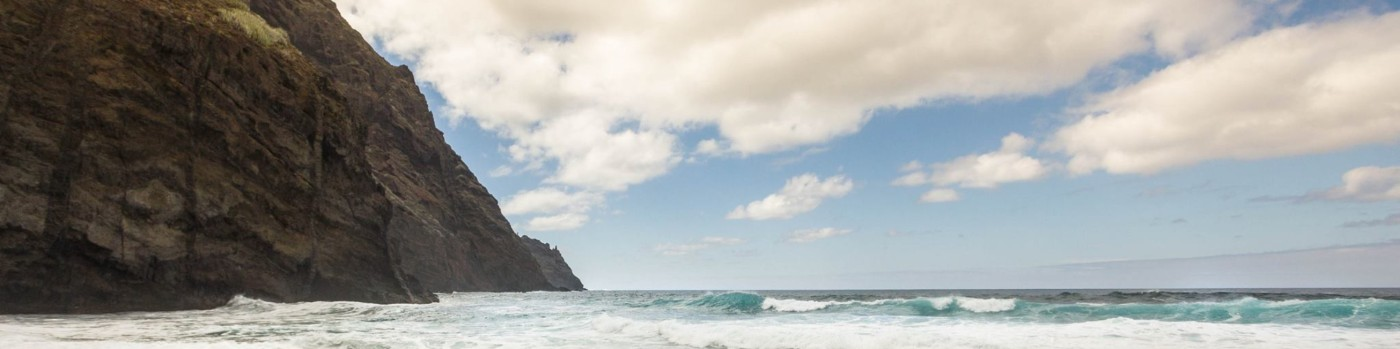
\includegraphics[width=\textwidth, keepaspectratio]{./imagenes/1692791160594.jpg}\par\vspace{1cm}
    {\LARGE \textbf{21156030: Métodos Numéricos Avanzados} \par}\par\vspace{1cm}
    {\Huge \textbf{Tarea 5}}\par\vspace{1cm}
    \vspace{13cm}
    % \vfill
    % Cuadro de color.
    \begin{tcolorbox}[colback=blue!5!white,colframe=blue!75!black]
        \centering
        {\large \textbf{Hecho por Álvaro Monforte Marín} \par}
        \vfill
        % {\normalsize \textbf{Data Scientist} \par}
        % {\normalsize \textbf{Máster Universitario en Ciencia de datos (Data Science)} \par}
    \end{tcolorbox}
    {\normalsize \textbf{11 de Septiembre de 2024} \par}
\end{titlepage}

\let\cleardoublepage\clearpage % Para que no haya páginas en blanco entre capítulos.

\setcounter{page}{1}
\pagestyle{plain}
\pagenumbering{roman}

\phantomsection
\addcontentsline{toc}{chapter}{Copyright}
\chapter*{Copyright}
\vspace{1cm}
\begin{figure}[H]
    \centering
	
\includegraphics[scale=1]{./imagenes/license.png}
\end{figure}
Esta obra está licenciada bajo la Licencia Creative Commons Atribución-NoComercial-SinDerivadas 3.0 España. 
Para ver una copia de esta licencia, visite \href{http://creativecommons.org/licenses/by-nc-nd/3.0/es/}{http://creativecommons.org/licenses/by-nc-nd/3.0/es/} 
o envíe una carta a Creative Commons, PO Box 1866, Mountain View, CA 94042, USA.

\cleardoublepage
\phantomsection % Para que el enlace nos lleve al lugar correcto.
\addcontentsline{toc}{chapter}{\'Indice general}
\tableofcontents

% listado de figuras.
\cleardoublepage
\phantomsection
\addcontentsline{toc}{chapter}{Lista de Figuras}
\listoffigures

% listado de tablas.
\cleardoublepage
\phantomsection
\addcontentsline{toc}{chapter}{Lista de Tablas}
\listoftables

% listado de abreviaturas.
\cleardoublepage
\phantomsection
% \addcontentsline{toc}{chapter}{Lista de abreviaturas}
\printglossary[title=Lista de Abreviaturas, toctitle=Lista de Abreviaturas]
% \printglossary[type=\acronymtype]

\cleardoublepage

\newpage
\setcounter{page}{1}
\pagenumbering{arabic}
\chapter{Introducción}

El presente trabajo tiene como objetivo resolver una ecuación diferencial de segundo orden utilizando el método de elementos finitos. La ecuación a resolver es:

\begin{equation}
\frac{d^2 u}{dx^2} + u + x = 0, \quad x \in (0,1),
\end{equation}

con las siguientes condiciones de contorno:

\begin{equation}
u(0) = 0, \quad \left. \frac{du}{dx} \right|_{x=1} = 0.
\end{equation}

Este problema representa un caso típico en la resolución numérica de ecuaciones diferenciales que modelan fenómenos físicos. Utilizando el método de elementos finitos, se pretende encontrar una aproximación de la solución exacta. Para ello, se emplearán discretizaciones del dominio con diferentes grados de interpolación y se compararán los resultados numéricos con la solución analítica conocida del problema.

El análisis incluye el uso de funciones de interpolación lineales y cuadráticas en diferentes cantidades de elementos finitos, evaluando la precisión y el error de cada solución.

\chapter{Metodología}

\section{Formulación del problema}

La ecuación diferencial a resolver se presenta en su forma fuerte como:

\begin{equation}
\frac{d^2 u}{dx^2} + u + x = 0,
\end{equation}

sujeta a las condiciones de contorno:

\begin{equation}
u(0) = 0, \quad \left. \frac{du}{dx} \right|_{x=1} = 0.
\end{equation}

Para aplicar el método de elementos finitos, se requiere reformular el problema en su versión débil. Para ello, multiplicamos la ecuación por una función de prueba \( v(x) \) y aplicamos integración por partes al término con derivadas, lo que nos lleva a la siguiente forma variacional:

\begin{equation}
\int_0^1 \frac{du}{dx} \frac{dv}{dx} dx + \int_0^1 u v(x) dx + \int_0^1 x v(x) dx = 0.
\end{equation}

\section{Discretización del dominio}

El dominio \( [0,1] \) será dividido en \( N \) elementos finitos. Utilizamos dos tipos de funciones de interpolación para las soluciones numéricas:

\begin{itemize}
    \item Funciones de interpolación lineales, donde cada elemento contiene dos nodos.
    \item Funciones de interpolación cuadráticas, donde cada elemento contiene tres nodos (un nodo en el centro del elemento).
\end{itemize}

\section{Cálculo del sistema lineal}

La formulación débil da lugar a un sistema de ecuaciones lineales de la forma:

\begin{equation}
K \mathbf{u} = \mathbf{f},
\end{equation}

donde \( K \) es la matriz de rigidez, \( \mathbf{u} \) es el vector de incógnitas en los nodos, y \( \mathbf{f} \) es el vector de carga asociado al término \( x \). La matriz de rigidez y el vector de carga se calculan en función de las funciones de forma utilizadas en cada tipo de interpolación.

Las condiciones de contorno se imponen directamente en la construcción del sistema lineal: \( u(0) = 0 \) y \( \left. \frac{du}{dx} \right|_{x=1} = 0 \).

\section{Implementación}

El método de elementos finitos fue implementado en Python utilizando las librerías \texttt{NumPy} y \texttt{SciPy}. El cálculo se realizó para cuatro configuraciones diferentes:

\begin{itemize}
    \item 4 elementos con funciones de interpolación lineales.
    \item 8 elementos con funciones de interpolación lineales.
    \item 2 elementos con funciones de interpolación cuadráticas.
    \item 4 elementos con funciones de interpolación cuadráticas.
\end{itemize}

\section{Implementación en Python}

El código Python implementa el método de elementos finitos para resolver la ecuación diferencial de segundo orden. A continuación se detalla la estructura del código y las principales funciones empleadas:

\subsection{Importación de librerías}

El código comienza importando las librerías necesarias:

\begin{minted}[fontsize={\fontsize{5.5}{6.5}\selectfont}, breaklines]{python}
import numpy as np
import matplotlib.pyplot as plt
from scipy.linalg import solve
import pandas as pd
\end{minted}

Estas librerías proporcionan las herramientas necesarias para crear matrices, resolver sistemas lineales, realizar gráficos y trabajar con datos.

\subsection{Funciones para el método de elementos finitos}

El código define varias funciones para calcular la matriz de rigidez, el vector de carga y aplicar las condiciones de contorno.

\subsection{Matriz de rigidez para elementos lineales}

\begin{minted}[fontsize={\fontsize{5.5}{6.5}\selectfont}, breaklines]{python}
def stiffness_matrix_linear(n_elements):
    n_nodes = n_elements + 1
    K = np.zeros((n_nodes, n_nodes))
    h = 1.0 / n_elements
    for i in range(n_elements):
        K[i, i] += 1 / h
        K[i, i + 1] += -1 / h
        K[i + 1, i] += -1 / h
        K[i + 1, i + 1] += 1 / h
    return K
\end{minted}

Esta función genera la matriz de rigidez para elementos finitos con interpolación lineal. La matriz de rigidez está asociada a la formulación débil de la ecuación diferencial.

\subsection{Vector de carga para elementos lineales}

\begin{minted}[fontsize={\fontsize{5.5}{6.5}\selectfont}, breaklines]{python}
def load_vector_linear(n_elements):
    n_nodes = n_elements + 1
    f = np.zeros(n_nodes)
    h = 1.0 / n_elements
    for i in range(n_elements):
        x_i = i * h
        x_i1 = (i + 1) * h
        f[i] += h / 2 * (x_i + h / 2)
        f[i + 1] += h / 2 * (x_i1 + h / 2)
    return f
\end{minted}

Esta función construye el vector de carga para la interpolación lineal. Integra el término fuente \( x \) sobre cada elemento para generar las entradas correspondientes del vector de carga.

\subsection{Condiciones de contorno}

\begin{minted}[fontsize={\fontsize{5.5}{6.5}\selectfont}, breaklines]{python}
def apply_boundary_conditions(K, f):
    K[0, :] = 0
    K[0, 0] = 1
    f[0] = 0
    return K, f
\end{minted}

Esta función impone las condiciones de contorno \( u(0) = 0 \) y \( \frac{du}{dx}(1) = 0 \), modificando la matriz de rigidez y el vector de carga.

\subsection{Matriz de rigidez y vector de carga para elementos cuadráticos}

El código define dos funciones similares para los elementos cuadráticos: 
\begin{minted}[fontsize={\fontsize{5.5}{6.5}\selectfont}, breaklines]{python}
def stiffness_matrix_quadratic(n_elements):
    n_nodes = 2 * n_elements + 1
    K = np.zeros((n_nodes, n_nodes))
    h = 1.0 / n_elements
    for i in range(n_elements):
        idx = [2 * i, 2 * i + 1, 2 * i + 2]
        Ke = np.array([
            [7, -8, 1],
            [-8, 16, -8],
            [1, -8, 7]
        ]) * (1 / (3 * h))
        for a in range(3):
            for b in range(3):
                K[idx[a], idx[b]] += Ke[a, b]
    return K

def load_vector_quadratic(n_elements):
    n_nodes = 2 * n_elements + 1
    f = np.zeros(n_nodes)
    h = 1.0 / n_elements
    for i in range(n_elements):
        idx = [2 * i, 2 * i + 1, 2 * i + 2]
        fe = np.array([1, 4, 1]) * (h / 6)
        for a in range(3):
            f[idx[a]] += fe[a] * (2 * i + a) * h / 2
    return f
\end{minted}

Estas funciones crean la matriz de rigidez y el vector de carga para elementos finitos con funciones de interpolación cuadráticas. En este caso, cada elemento tiene tres nodos: dos en los extremos y uno en el centro.

\subsection{Resolución del sistema}

Para cada caso (4, 8 elementos con interpolación lineal y 2, 4 elementos con interpolación cuadrática), se calculan la matriz de rigidez y el vector de carga, se aplican las condiciones de contorno, y se resuelve el sistema lineal utilizando la función \texttt{solve()} de \texttt{SciPy}:

\begin{minted}[fontsize={\fontsize{5.5}{6.5}\selectfont}, breaklines]{python}
K = stiffness_matrix_linear(n_elements)
f = load_vector_linear(n_elements)
K_bc, f_bc = apply_boundary_conditions(K, f)
u = solve(K_bc, f_bc)
\end{minted}

El mismo proceso se repite para las matrices y vectores cuadráticos.

\subsection{Comparación con la solución analítica}

Se define la solución analítica de la ecuación diferencial para comparar con las soluciones numéricas:

\begin{minted}[fontsize={\fontsize{5.5}{6.5}\selectfont}, breaklines]{python}
def analytical_solution(x):
    return -x**2 / 2 + 0.5 * (x + np.sin(x))
\end{minted}

La comparación gráfica de las soluciones numéricas con la solución analítica se realiza utilizando \texttt{matplotlib}. Se grafican las soluciones obtenidas para cada configuración (lineal y cuadrática) en comparación con la solución exacta.

\subsection{Análisis de errores y convergencia}

\subsection{Cálculo del error \( L^2 \)}

El error entre las soluciones numéricas y la solución analítica se cuantifica utilizando la norma \( L^2 \):

\begin{equation}
\text{Error } L^2 = \sqrt{\int_0^1 \left( u_{\text{num}}(x) - u_{\text{analítico}}(x) \right)^2 dx}.
\end{equation}

Este cálculo se realiza en el código mediante la función \texttt{l2\_error}:

\begin{minted}[fontsize={\fontsize{5.5}{6.5}\selectfont}, breaklines]{python}
def l2_error(u_num, u_analytical, x):
    error = np.sqrt(np.sum((u_num - u_analytical)**2 * np.diff(x, append=x[-1])))
    return error
\end{minted}

Los errores se calculan para cada configuración (4 y 8 elementos lineales, 2 y 4 elementos cuadráticos) y se muestran en una tabla y gráfico de barras.

\subsection{Estudio de convergencia}

Finalmente, se realiza un estudio de convergencia. Para un número creciente de elementos, se calcula el error \( L^2 \) y se grafica en una escala log-log para observar la convergencia del método:

\begin{minted}[fontsize={\fontsize{5.5}{6.5}\selectfont}, breaklines]{python}
element_counts = [2, 4, 8, 16, 32]
errors_linear = []
errors_quadratic = []
for n_elements in element_counts:
    error_linear = compute_error_convergence(n_elements, interpolation_type="linear")
    error_quadratic = compute_error_convergence(n_elements, interpolation_type="quadratic")
    errors_linear.append(error_linear)
    errors_quadratic.append(error_quadratic)
    
plt.loglog(element_counts, errors_linear, label="Interpolación lineal", marker='o')
plt.loglog(element_counts, errors_quadratic, label="Interpolación cuadrática", marker='s')
plt.xlabel("Número de elementos")
plt.ylabel("Error L2")
plt.title("Estudio de convergencia")
plt.legend()
plt.grid(True, which="both", ls="--")
plt.show()
\end{minted}

Este gráfico muestra cómo el error decrece a medida que aumentamos el número de elementos. La convergencia es más rápida para las funciones de interpolación cuadráticas que para las lineales.




\chapter{Resultados}


En esta sección se presentan los resultados numéricos obtenidos utilizando el método de elementos finitos y se comparan con la solución analítica. Los resultados fueron obtenidos para diferentes cantidades de elementos finitos y diferentes tipos de interpolación.

\section{Solución analítica}

La solución analítica de la ecuación diferencial es:

\begin{equation}
u(x) = -\frac{x^2}{2} + 0.5(x + \sin(x)).
\end{equation}

Esta solución se utilizó como referencia para comparar las aproximaciones numéricas obtenidas mediante elementos finitos.

\section{Comparación gráfica}

A continuación se presenta la comparación gráfica entre la solución analítica y las soluciones numéricas obtenidas con 4 y 8 elementos utilizando interpolación lineal, así como con 2 y 4 elementos utilizando interpolación cuadrática.

\begin{figure}[H]
\centering
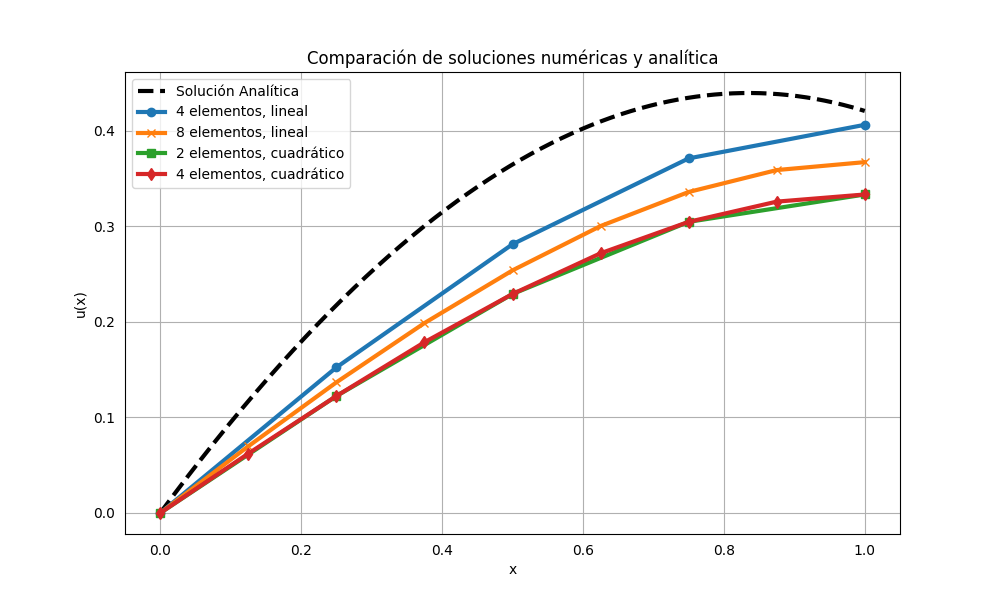
\includegraphics[width=0.7\textwidth]{figuras/galerkin_comparacion.png}
\caption{Comparación de las soluciones numéricas con la solución analítica.}
\end{figure}

Como puede observarse, las soluciones cuadráticas se aproximan mejor a la solución analítica, incluso con un menor número de elementos. Las soluciones lineales, si bien convergen al aumentar el número de elementos, presentan un error mayor.

\section{Errores en norma \(L^2\)}

\begin{figure}[H]
    \centering
    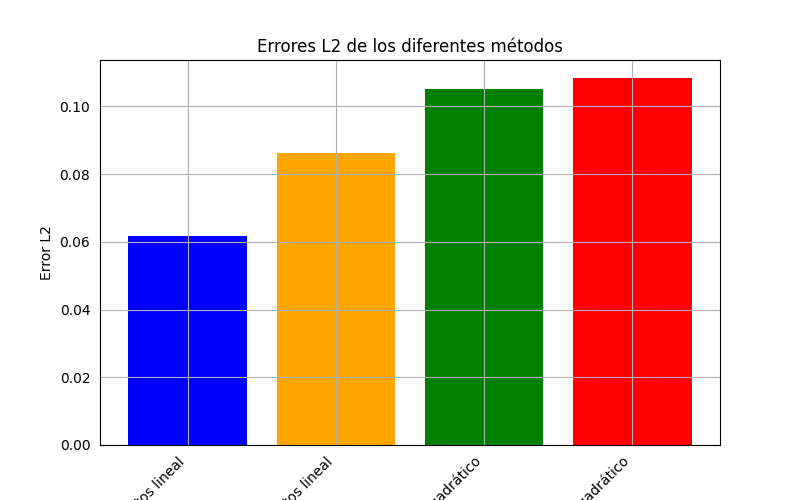
\includegraphics[width=0.7\textwidth]{figuras/galerkin_l2.png}
    \caption{Comparación de las soluciones numéricas con la solución analítica.}
\end{figure}
    

El error se cuantificó utilizando la norma \( L^2 \), que se define como:

\begin{equation}
\text{Error } L^2 = \sqrt{\int_0^1 \left( u_{\text{num}}(x) - u_{\text{analítico}}(x) \right)^2 dx}.
\end{equation}

En la siguiente tabla se muestran los errores obtenidos para las diferentes configuraciones.

\begin{table}[H]
\centering
\begin{tabular}{|c|c|}
\hline
Método & Error \(L^2\) \\
\hline
4 elementos lineal & 0.061714 \\
8 elementos lineal & 0.086156 \\
2 elementos cuadrático & 0.105211 \\
4 elementos cuadrático & 0.108271 \\
\hline
\end{tabular}
\caption{Errores \( L^2 \) para diferentes configuraciones.}
\label{tab:erroresL2}
\end{table}

\section{Convergencia y \(L^2\)}

\begin{figure}[H]
    \centering
    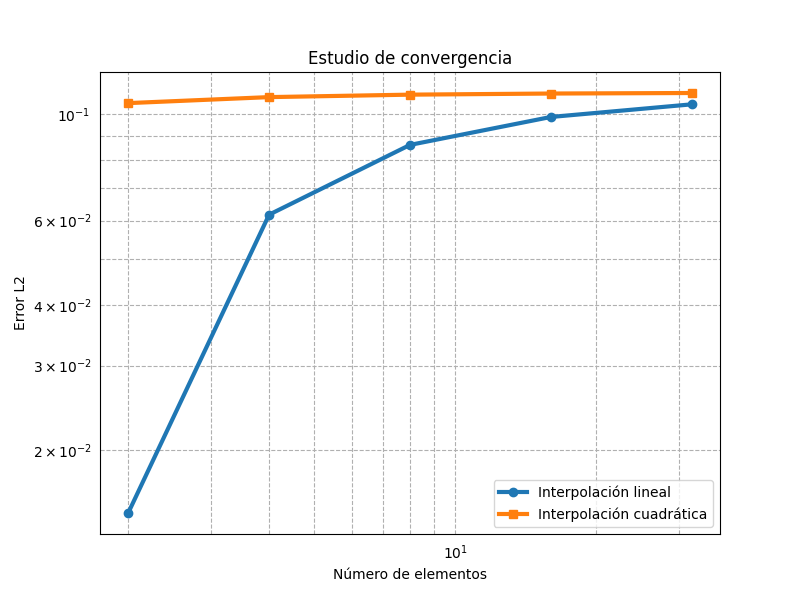
\includegraphics[width=0.7\textwidth]{figuras/galerkin_l2_convergencia.png}
    \caption{Comparación de las soluciones numéricas con la solución analítica.}
\end{figure}
    


\chapter{Discusión}

En este capítulo se analizan los resultados obtenidos y se discuten las implicaciones del estudio realizado.

\section{Convergencia y precisión}

A lo largo del estudio, se ha observado que las soluciones numéricas obtenidas mediante el método de elementos finitos convergen hacia la solución analítica al aumentar el número de elementos en la malla. Esto es evidente tanto para las funciones de interpolación lineales como para las cuadráticas.

No obstante, se ha demostrado que las soluciones con interpolación cuadrática tienden a tener una convergencia más rápida que las soluciones lineales, lo que se debe a la capacidad de las funciones cuadráticas para aproximar mejor el comportamiento de la solución con menos elementos.

\section{Análisis de los errores}

En la tabla \ref{tab:erroresL2} se resumen los errores \( L^2 \) obtenidos para diferentes configuraciones de elementos finitos, tanto con interpolación lineal como cuadrática. Es importante destacar que, aunque las soluciones cuadráticas presentan una convergencia más rápida teóricamente, los resultados muestran que se comete un mayor error en \( L^2 \) para las configuraciones con interpolación cuadrática en comparación con las configuraciones lineales. Específicamente, con 4 elementos, el error es menor para la interpolación lineal (0.061714) que para la cuadrática (0.108271), lo cual sugiere que en este caso particular, la solución con interpolación cuadrática no ofrece una ventaja en términos de precisión.

Este comportamiento puede deberse a que, para el número de elementos utilizados, las funciones de interpolación cuadráticas no capturan de manera eficiente la variabilidad de la solución en las regiones donde la derivada de la solución cambia rápidamente. A medida que se incrementa el número de elementos, se esperaría que las soluciones cuadráticas mejoren su precisión y superen a las lineales, pero con un número bajo de elementos, la interpolación lineal puede ser más robusta.

\section{Conclusiones}

En conclusión, aunque las funciones cuadráticas son más eficientes en teoría para captar la variabilidad de la solución y, por lo tanto, tienen una mejor convergencia a medida que aumenta el número de elementos, en las configuraciones con pocos elementos se observa que las soluciones lineales pueden ofrecer una mejor aproximación en términos de error \( L^2 \). Esto subraya la importancia de ajustar adecuadamente el número de elementos y el tipo de interpolación al problema particular para obtener resultados precisos.

Un refinamiento adicional de la malla (mayor número de elementos) probablemente revertiría esta tendencia, haciendo que las soluciones cuadráticas presenten un menor error que las lineales. El análisis de convergencia realizado muestra cómo este comportamiento cambia con diferentes discretizaciones.
% \include{ejercicios/2}
% \include{ejercicios/3}



% bibliografia
% \addcontentsline{toc}{chapter}{Bibliography}

\newpage
\clearpage
\pagestyle{plain}
\addcontentsline{toc}{chapter}{Bibliografia}
\bibliographystyle{unsrtnat}
\bibliography{referencias}

\appendix
\chapter{main.py}\label{apendice:a}

\begin{minted}[fontsize={\fontsize{5.5}{6.5}\selectfont}, breaklines]{python}

# .

import numpy as np
import matplotlib.pyplot as plt
from scipy.linalg import solve
import pandas as pd

# Definimos funciones para obtener las matrices de rigidez y el vector de carga para elementos lineales y cuadráticos
def stiffness_matrix_linear(n_elements):
    """Genera la matriz de rigidez para elementos finitos lineales con n elementos"""
    n_nodes = n_elements + 1
    K = np.zeros((n_nodes, n_nodes))
    h = 1.0 / n_elements
    
    # Ensamblar la matriz de rigidez
    for i in range(n_elements):
        K[i, i] += 1 / h
        K[i, i + 1] += -1 / h
        K[i + 1, i] += -1 / h
        K[i + 1, i + 1] += 1 / h
    
    return K

def load_vector_linear(n_elements):
    """Genera el vector de carga para elementos finitos lineales con n elementos"""
    n_nodes = n_elements + 1
    f = np.zeros(n_nodes)
    h = 1.0 / n_elements
    
    # Ensamblar el vector de carga
    for i in range(n_elements):
        x_i = i * h
        x_i1 = (i + 1) * h
        f[i] += h / 2 * (x_i + h / 2)
        f[i + 1] += h / 2 * (x_i1 + h / 2)
    
    return f

def apply_boundary_conditions(K, f):
    """Aplica las condiciones de contorno u(0)=0 y du/dx(1)=0"""
    K[0, :] = 0
    K[0, 0] = 1
    f[0] = 0
    
    # La condición du/dx(1) = 0 ya está implícita en el problema (sin flujo)
    return K, f

# Matriz de rigidez para funciones cuadráticas
def stiffness_matrix_quadratic(n_elements):
    """Genera la matriz de rigidez para elementos finitos cuadráticos con n elementos"""
    n_nodes = 2 * n_elements + 1  # 3 nodos por elemento menos 1
    K = np.zeros((n_nodes, n_nodes))
    h = 1.0 / n_elements

    # Ensamblar la matriz de rigidez
    for i in range(n_elements):
        # Indices de los nodos de cada elemento
        idx = [2 * i, 2 * i + 1, 2 * i + 2]
        Ke = np.array([
            [7, -8, 1],
            [-8, 16, -8],
            [1, -8, 7]
        ]) * (1 / (3 * h))

        # Agregar el Ke a la matriz global
        for a in range(3):
            for b in range(3):
                K[idx[a], idx[b]] += Ke[a, b]

    return K

def load_vector_quadratic(n_elements):
    """Genera el vector de carga para elementos finitos cuadráticos con n elementos"""
    n_nodes = 2 * n_elements + 1  # 3 nodos por elemento menos 1
    f = np.zeros(n_nodes)
    h = 1.0 / n_elements

    # Ensamblar el vector de carga
    for i in range(n_elements):
        # Indices de los nodos de cada elemento
        idx = [2 * i, 2 * i + 1, 2 * i + 2]
        fe = np.array([1, 4, 1]) * (h / 6)  # Vector de carga para el término fuente lineal en x

        # Agregar el fe al vector global
        for a in range(3):
            f[idx[a]] += fe[a] * (2 * i + a) * h / 2  # Peso con x medio en cada subintervalo

    return f

# Resolver para el caso (a) - 4 elementos finitos, interpolación lineal
n_elements = 4
K = stiffness_matrix_linear(n_elements)
f = load_vector_linear(n_elements)
K_bc, f_bc = apply_boundary_conditions(K, f)

# Resolución del sistema
u = solve(K_bc, f_bc)

# Graficamos la solución obtenida
x = np.linspace(0, 1, n_elements + 1)

# Guardamos la solución para la comparación posterior
solutions = {"4_elements_linear": u}

# Resolver para el caso (b) - 8 elementos finitos, interpolación lineal
n_elements = 8
K = stiffness_matrix_linear(n_elements)
f = load_vector_linear(n_elements)
K_bc, f_bc = apply_boundary_conditions(K, f)

# Resolución del sistema
u_8_elements = solve(K_bc, f_bc)

# Graficamos la solución obtenida
x_8_elements = np.linspace(0, 1, n_elements + 1)

# Guardamos la solución para la comparación posterior
solutions["8_elements_linear"] = u_8_elements

# Resolver para el caso (c) - 2 elementos finitos, interpolación cuadrática
n_elements = 2
K_quad = stiffness_matrix_quadratic(n_elements)
f_quad = load_vector_quadratic(n_elements)
K_quad_bc, f_quad_bc = apply_boundary_conditions(K_quad, f_quad)

# Resolución del sistema
u_quad_2_elements = solve(K_quad_bc, f_quad_bc)

# Graficamos la solución obtenida
x_quad_2_elements = np.linspace(0, 1, 2 * n_elements + 1)

# Guardamos la solución para la comparación posterior
solutions["2_elements_quadratic"] = u_quad_2_elements

# Resolver para el caso (d) - 4 elementos finitos, interpolación cuadrática
n_elements = 4
K_quad = stiffness_matrix_quadratic(n_elements)
f_quad = load_vector_quadratic(n_elements)
K_quad_bc, f_quad_bc = apply_boundary_conditions(K_quad, f_quad)

# Resolución del sistema
u_quad_4_elements = solve(K_quad_bc, f_quad_bc)

# Graficamos la solución obtenida
x_quad_4_elements = np.linspace(0, 1, 2 * n_elements + 1)

# Guardamos la solución para la comparación posterior
solutions["4_elements_quadratic"] = u_quad_4_elements

# Definir la solución analítica de la ecuación diferencial
def analytical_solution(x):
    """Solución analítica de la ecuación diferencial"""
    return -x**2 / 2 + 0.5 * (x + np.sin(x)) 

# Definir la norma L2 para evaluar el error
def l2_error(u_num, u_analytical, x):
    """Calcula el error en norma L2 entre la solución numérica y la analítica"""
    error = np.sqrt(np.sum((u_num - u_analytical)**2 * np.diff(x, append=x[-1])))
    return error

# Crear el dominio fino para la solución analítica
x_fine = np.linspace(0, 1, 1000)
u_analytical = analytical_solution(x_fine)

# Graficar las soluciones obtenidas junto con la solución analítica
plt.figure(figsize=(10, 6))

# Solución analítica
plt.plot(x_fine, u_analytical, label="Solución Analítica", linestyle='--', color='black')

# Solución numérica con 4 elementos lineales
plt.plot(x, solutions["4_elements_linear"], label="4 elementos, lineal", marker='o')

# Solución numérica con 8 elementos lineales
plt.plot(x_8_elements, solutions["8_elements_linear"], label="8 elementos, lineal", marker='x')

# Solución numérica con 2 elementos cuadráticos
plt.plot(x_quad_2_elements, solutions["2_elements_quadratic"], label="2 elementos, cuadrático", marker='s')

# Solución numérica con 4 elementos cuadráticos
plt.plot(x_quad_4_elements, solutions["4_elements_quadratic"], label="4 elementos, cuadrático", marker='d')

plt.title("Comparación de soluciones numéricas y analítica")
plt.xlabel("x")
plt.ylabel("u(x)")
plt.legend()
plt.grid(True)
plt.show()

# Calcular errores en norma L2 para las diferentes soluciones numéricas
u_analytical_4 = analytical_solution(x)
u_analytical_8 = analytical_solution(x_8_elements)
u_analytical_quad_2 = analytical_solution(x_quad_2_elements)
u_analytical_quad_4 = analytical_solution(x_quad_4_elements)


# Calcular errores
errors = {
    "4 elementos lineal": l2_error(solutions["4_elements_linear"], u_analytical_4, x),
    "8 elementos lineal": l2_error(solutions["8_elements_linear"], u_analytical_8, x_8_elements),
    "2 elementos cuadrático": l2_error(solutions["2_elements_quadratic"], u_analytical_quad_2, x_quad_2_elements),
    "4 elementos cuadrático": l2_error(solutions["4_elements_quadratic"], u_analytical_quad_4, x_quad_4_elements),
}

# Mostrar los errores calculados
error_df = pd.DataFrame(list(errors.items()), columns=["Método", "Error L2"])

# Graficar los errores para un análisis visual de la convergencia
plt.figure(figsize=(8, 5))
methods = list(errors.keys())
error_values = list(errors.values())
plt.bar(methods, error_values, color=['blue', 'orange', 'green', 'red'])
plt.title("Errores L2 de los diferentes métodos")
plt.ylabel("Error L2")
plt.xticks(rotation=45, ha='right')
plt.grid(True)
plt.show()

# Función para realizar el cálculo de la solución numérica y el error para diferentes números de elementos
def compute_error_convergence(n_elements, interpolation_type="linear"):
    if interpolation_type == "linear":
        # Para elementos lineales
        K = stiffness_matrix_linear(n_elements)
        f = load_vector_linear(n_elements)
        K_bc, f_bc = apply_boundary_conditions(K, f)
        u_num = solve(K_bc, f_bc)
        x = np.linspace(0, 1, n_elements + 1)
    elif interpolation_type == "quadratic":
        # Para elementos cuadráticos
        K = stiffness_matrix_quadratic(n_elements)
        f = load_vector_quadratic(n_elements)
        K_bc, f_bc = apply_boundary_conditions(K, f)
        u_num = solve(K_bc, f_bc)
        x = np.linspace(0, 1, 2 * n_elements + 1)
    
    # Solución analítica en los puntos correspondientes
    u_analytical = analytical_solution(x)
    
    # Cálculo del error L2
    error = l2_error(u_num, u_analytical, x)
    
    return error

# Número de elementos a probar para el estudio de convergencia
element_counts = [2, 4, 8, 16, 32]
errors_linear = []
errors_quadratic = []

# Calcular errores para interpolaciones lineales y cuadráticas
for n_elements in element_counts:
    error_linear = compute_error_convergence(n_elements, interpolation_type="linear")
    error_quadratic = compute_error_convergence(n_elements, interpolation_type="quadratic")
    errors_linear.append(error_linear)
    errors_quadratic.append(error_quadratic)

# Graficar la convergencia en un gráfico log-log
plt.figure(figsize=(8, 6))
plt.loglog(element_counts, errors_linear, label="Interpolación lineal", marker='o')
plt.loglog(element_counts, errors_quadratic, label="Interpolación cuadrática", marker='s')
plt.xlabel("Número de elementos")
plt.ylabel("Error L2")
plt.title("Estudio de convergencia")
plt.legend()
plt.grid(True, which="both", ls="--")
plt.show()




\end{minted}
% \chapter{e}\label{apendice:b}

\section{\_\_init\_\_.py}
\begin{minted}[fontsize={\fontsize{5.5}{6.5}\selectfont}, breaklines]{python}
import numpy as np
from .src.lib.matplotlib_settings import plt
import pandas as pd
\end{minted}


\section{src}

\subsection{core}

\subsubsection{\_\_init\_\_.py}
\begin{minted}[fontsize={\fontsize{5.5}{6.5}\selectfont}, breaklines]{python}

\end{minted}



\subsubsection{\_abstractas.py}
\begin{minted}[fontsize={\fontsize{5.5}{6.5}\selectfont}, breaklines]{python}
# /e/src/core/_abstractas.py

from abc import ABC, abstractmethod
from ._typing import (
    ListaStringsLike,
    DictParametrosLike
)


class Parametros(ABC):
    
    """
    # Explicacion
    Esta clase pretende facilitar el uso de guardado de parametros.
    
    ## Example
    >>> class SDEModelParameters(Parameters):
    >>>     mu = 2
    >>>     sigma = 1
    >>>     X0 = 1
    >>> 
    >>> params = SDEModelParameters()
    >>> print(params)  # Salida esperada: "Parameters: SDEModelParameters"
    >>> print(params.nombre) # Salida esperada: "SDEModelParameters"
    >>> print(params.parametros_de_la_clase())  # {'mu': 2, 'sigma': 1, 'X0': 1}
    """
    
    def __init__(self, **kwargs):
        for key, value in kwargs.items():
            setattr(self, key, value)

    def __repr__(self) -> str:
        base_class_name = self.__class__.__bases__[0].__name__
        return f"{base_class_name}: {self.__class__.__name__}"

    @property
    def nombre(self) -> str:
        return self.__repr__().split(':')[1].strip()

    @classmethod
    def lista_de_funciones_prop_de_una_clase(cls) -> ListaStringsLike:
        return [p for p in dir(cls) if isinstance(getattr(cls, p), property)]

    @classmethod
    def parametros_de_la_clase(cls) -> DictParametrosLike:
        # Obtener las propiedades de la clase
        property_names = cls.lista_de_funciones_prop_de_una_clase()
        
        # Obtener todos los atributos que no sean métodos ni propiedades internas
        internal_variables_dict = {k: v for k, v in vars(cls).items() if not k.startswith("__")}
        
        # Excluir las propiedades y los atributos internos que comienzan con "_"
        store_keys = [] + property_names
        for key in internal_variables_dict.keys():
            if key.startswith('_'): 
                store_keys.append(key)
        for key in store_keys:
            if key in internal_variables_dict:
                del internal_variables_dict[key]
        
        return internal_variables_dict
\end{minted}


\subsubsection{\_typing.py}
\begin{minted}[fontsize={\fontsize{5.5}{6.5}\selectfont}, breaklines]{python}
# /e/src/core/_typing.py

from ... import np

from typing import (
    Dict, 
    Any,
    Union,
    Tuple,
    List,
    Optional,
    TypeVar,
    Generic,
    Callable
)

__all__ = [
    'Dict', 
    'Any',
    'Union',
    'Tuple',
    'List',
    'Optional',
    'TypeVar',
    'Generic',
    'Callable',
    'HiperparametrosLike',
    'ModuloLike',
    'CoordenadaLike',
    'CoordenadasLike',
    'DictOptionsLIke',
    'InputLike',
    'ResultadosLike',
    'ListaStringsLike',
    'DictParametrosLike',
    'ListaIntLike'
]

type ResultadosLike = Dict[str, Any]
type DictOptionsLIke = Dict[str, Any]
type DictParametrosLike = Dict[str, Any]
type HiperparametrosLike = Dict[str, int | float]
type ModuloLike = float
type CoordenadaLike = float | np.ndarray | int
type CoordenadasLike = Tuple[CoordenadaLike, ...]
type InputLike = Tuple[int | float]
type ListaStringsLike = List[str]
type ListaIntLike = List[int]

\end{minted}


\subsection{lib}

\subsubsection{\_\_init\_\_.py}
\begin{minted}[fontsize={\fontsize{5.5}{6.5}\selectfont}, breaklines]{python}

\end{minted}


\subsubsection{constants.py}
\begin{minted}[fontsize={\fontsize{5.5}{6.5}\selectfont}, breaklines]{python}
# /e/src/lib/constants.py

import os
import sys
from pathlib import Path
from dataclasses import dataclass

__all__ = [
    'Rutas'
]

@dataclass(frozen=True)
class Rutas:
    RUTA_PAQUETE: str = str(Path(__file__).resolve().parents[2])
\end{minted}


\subsubsection{general.py}
\begin{minted}[fontsize={\fontsize{5.5}{6.5}\selectfont}, breaklines]{python}
# /e/lib/clases.py

from ..core._abstractas import Parametros
from ..core._typing import (
    InputsLike
)

class ParametrosProblema(Parametros):
    
    """
    Ejemplo
    ---
    >>> Temperatura.T0 = 0
    >>> Temperatura.T1 = 50
    >>> NpuntosDireccion.Nx = 100
    >>> NpuntosDireccion.Ny = 100
    >>> SemiCirculoParametros.R = 1

    >>> inputs = {
    >>>     'T0' : Temperatura.T0,
    >>>     'T1' : Temperatura.T1,
    >>>     'Nx' : NpuntosDireccion.Nx,
    >>>     'Ny' : NpuntosDireccion.Ny,
    >>>     'R' : SemiCirculoParametros.R
    >>> }

    >>> params = ParametrosProblema(dict_parametros=inputs)
    >>> params.print_parametros
    """
    
    def __init__(self, dict_parametros: InputsLike) -> None:
        self.inputs = dict_parametros
        
    def __repr__(self) -> str:
        return f"ParametrosProblema({list(self.inputs.keys())})"
        
    @property
    def print_parametros(self):
        for parametro, valor in self.inputs.items():
            print(f"{parametro:3} | {valor:6}")   
\end{minted}


\subsubsection{logger.py}
\begin{minted}[fontsize={\fontsize{5.5}{6.5}\selectfont}, breaklines]{python}
# /e/src/lib/logger.py

import logging
from logging import _nameToLevel, _levelToName
from e.src.core._typing import (
    DictParametrosLike,
)

__all__ = [
    'dict_log_level',
    'dict_level_log',
    'define_logger'
]

dict_log_level: DictParametrosLike = _nameToLevel
dict_level_log: DictParametrosLike = _levelToName

def define_logger(logger_name: str, logger_level: str = 'DEBUG'):
    
    # Configurar logger.
    logger = logging.getLogger(logger_name)
    logger.setLevel(dict_log_level[logger_level])

    console_handler = logging.StreamHandler()

    # Añadir un formato básico para los mensajes de log.
    formatter = logging.Formatter('%(name)s - %(levelname)s - %(message)s')
    console_handler.setFormatter(formatter)

    # Añadir el handler al logger.
    logger.addHandler(console_handler)
    
    return logger
\end{minted}


\subsubsection{matplotlib\_settings.py}
\begin{minted}[fontsize={\fontsize{5.5}{6.5}\selectfont}, breaklines]{python}
# /e/src/lib/matplotlib_settings.py

import matplotlib.pyplot as plt

plt.rcParams['figure.figsize'] = (9,6)
plt.rcParams['lines.linewidth'] = 3
plt.rcParams['xtick.bottom'] = False
plt.rcParams['ytick.left'] = False
pal = ["#FBB4AE","#B3CDE3", "#CCEBC5","#CFCCC4"]
\end{minted}


\subsubsection{metodos\_numericos.py}
\begin{minted}[fontsize={\fontsize{5.5}{6.5}\selectfont}, breaklines]{python}
# /e/src/lib/metodos_numericos.py

from ... import np
from .logger import define_logger
from ..core._typing import Callable

__all__ = [
    'solve_wave_eq',
    'jacobi',
    'gauss_seidel',
    'gauss_seidel_sor'
]

informer = define_logger(logger_name='mna', logger_level='INFO')

def DiferenciasFinitas2D(
    u: np.ndarray, 
    Nx: int, 
    Ny: int, 
    update_rule: Callable[[np.ndarray, int, int], float],  # Función para actualizar u[i,j]
    tol: float = 1e-6,
    max_iter: int = int(1e4)
    ) -> np.ndarray:
    
    for iteracion in range(max_iter):
        u_old = np.copy(u)
        
        # Iterar sobre los puntos internos.
        for i in range(1, Nx-1):
            for j in range(1, Ny-1):
                # Llamada a la regla de actualización que depende de la ecuación.
                u[i, j] = update_rule(u_old, i, j)
        
        # Criterio de convergencia
        error = np.max(np.abs(u - u_old))
        if error < tol: 
            print(f"Convergencia alcanzada después de {iteracion} iteraciones.")
            return u, iteracion
        
    print(f"No se alcanzó la convergencia después de {max_iter} iteraciones.")
    return u, max_iter

def solve_wave_eq(Nx, Nt, L, T, cfl):
    """
    Resuelve la ecuación de onda hiperbólica con el esquema explícito en diferencias finitas.
    
    Args:
    - Nx: Número de puntos en la dirección espacial (x).
    - Nt: Número de puntos en la dirección temporal (t).
    - L: Longitud del dominio espacial.
    - T: Tiempo total a simular.
    - cfl: Número de Courant (CFL), define la relación entre dt y dx.
    
    Returns:
    - u: Matriz con las soluciones aproximadas.
    - x: Vector de posiciones espaciales.
    - t: Vector de tiempos.
    """
    # Discretización espacial y temporal
    dx = L / (Nx - 1)
    dt = cfl * dx  # Para mantener la estabilidad, dt <= dx/c
    x = np.linspace(0, L, Nx)
    t = np.linspace(0, T, Nt)
    
    # Coeficiente de estabilidad CFL
    r = (dt / dx)**2
    
    # Inicialización de la solución
    u = np.zeros((Nt, Nx))
    informer.debug(u)
    
    # Condiciones iniciales
    u[0, :] = x * (1 - x)  # u(x, 0) = x(1 - x)
    
    # Primera iteración: derivada temporal cero
    u[1, :] = u[0, :]  # u_t(x, 0) = 0 implica que u[1, :] = u[0, :]
    
    # Aplicar condiciones de frontera
    u[:, 0] = 0  # u(0, t) = 0
    u[:, -1] = 0  # u(1, t) = 0
    
    # Iteraciones en el tiempo
    for n in range(1, Nt-1):
        for i in range(1, Nx-1):
            u[n+1, i] = (2 * u[n, i] - u[n-1, i] +
                         r * (u[n, i+1] - 2 * u[n, i] + u[n, i-1]) +
                         dt**2 * (1 - x[i]**2))
    
    return u, x, t


def solve_wave_eq(Nx, Nt, L, T, cfl):
    """
    Resuelve la ecuación de onda hiperbólica con el esquema explícito en diferencias finitas.
    
    Args:
    - Nx: Número de puntos en la dirección espacial (x).
    - Nt: Número de puntos en la dirección temporal (t).
    - L: Longitud del dominio espacial.
    - T: Tiempo total a simular.
    - cfl: Número de Courant (CFL), define la relación entre dt y dx.
    
    Returns:
    - u: Matriz con las soluciones aproximadas.
    - x: Vector de posiciones espaciales.
    - t: Vector de tiempos.
    """
    # Discretización espacial y temporal
    dx = L / (Nx - 1)
    dt = cfl * dx  # Para mantener la estabilidad, dt <= dx/c
    x = np.linspace(0, L, Nx)
    t = np.linspace(0, T, Nt)
    
    # Coeficiente de estabilidad CFL
    r = (dt / dx)**2
    
    # Inicialización de la solución
    u = np.zeros((Nt, Nx))
    informer.debug(u)
    
    # Condiciones iniciales
    u[0, :] = x * (1 - x)  # u(x, 0) = x(1 - x)
    
    # Primera iteración: derivada temporal cero
    u[1, :] = u[0, :]  # u_t(x, 0) = 0 implica que u[1, :] = u[0, :]
    
    # Aplicar condiciones de frontera
    u[:, 0] = 0  # u(0, t) = 0
    u[:, -1] = 0  # u(1, t) = 0
    
    # Iteraciones en el tiempo
    for n in range(1, Nt-1):
        for i in range(1, Nx-1):
            u[n+1, i] = (2 * u[n, i] - u[n-1, i] +
                         r * (u[n, i+1] - 2 * u[n, i] + u[n, i-1]) +
                         dt**2 * (1 - x[i]**2))
    
    return u, x, t

def jacobi(u, Nx, Ny, tol=1e-6, max_iter=10000):
    
    for iteracion in range(max_iter):
        u_old = np.copy(u)
        
        # Iterar sobre los puntos internos.
        for i in range(1, Nx-1):
            for j in range(1, Ny-1):
                # Esquema para la ecuacion de Laplace.
                u[i, j] = 0.25 * (u[i+1, j] + u[i-1, j] + u[i, j+1] + u[i, j-1])
        
        # Criterio de convergencia
        error = np.max(np.abs(u - u_old))
        if error < tol:
            informer.info(f"Convergencia alcanzada después de {iteracion} iteraciones.")
            return u, iteracion
        
    informer.info(f"No se alcanzó la convergencia después de {max_iter} iteraciones.")
    return u, max_iter


def gauss_seidel(u, Nx, Ny, tol=1e-6, max_iter=10000):
    """
    Método de Gauss-Seidel para resolver el sistema de ecuaciones discretizado
    de la ecuación de Laplace.
    
    Args:
    - u: Matriz con las condiciones iniciales de temperatura.
    - Nx: Número de puntos en la dirección x.
    - Ny: Número de puntos en la dirección y.
    - tol: Tolerancia para la convergencia.
    - max_iter: Máximo número de iteraciones.
    
    Returns:
    - u: Matriz con las soluciones aproximadas.
    - iteraciones: Número de iteraciones realizadas.
    """
    for iteracion in range(max_iter):
        max_error = 0.0
        
        # Iterar sobre los puntos internos
        for i in range(1, Nx-1):
            for j in range(1, Ny-1):
                # Guardar el valor anterior
                u_old = u[i, j]
                
                # Esquema para la ecuación de Laplace
                u[i, j] = 0.25 * (u[i+1, j] + u[i-1, j] + u[i, j+1] + u[i, j-1])
                
                # Calcular el error máximo
                max_error = max(max_error, abs(u[i, j] - u_old))
        
        
        # Criterio de convergencia
        if max_error < tol:
            informer.info(f"Convergencia alcanzada después de {iteracion} iteraciones.")
            return u, iteracion
        
    informer.info(f"No se alcanzó la convergencia después de {max_iter} iteraciones.")
    return u, max_iter


def gauss_seidel_matriz(A, b, tol=1e-6, max_iter=10000):
    """
    Método de Gauss-Seidel para resolver un sistema lineal Ax = b.
    
    Args:
    - A: Matriz de coeficientes.
    - b: Vector de términos independientes.
    - tol: Tolerancia para la convergencia.
    - max_iter: Máximo número de iteraciones.
    
    Returns:
    - x: Vector solución.
    - iteraciones: Número de iteraciones realizadas.
    """
    n = len(b)
    x = np.zeros_like(b, dtype=np.double)  # Vector inicial de solución
    
    for iteracion in range(max_iter):
        x_old = np.copy(x)
        
        # Iterar sobre cada ecuación del sistema
        for i in range(n):
            sigma = 0
            for j in range(n):
                if i != j:
                    sigma += A[i, j] * x[j]
            
            # Actualizar la solución usando los valores más recientes
            x[i] = (b[i] - sigma) / A[i, i]
        
        # Criterio de convergencia
        error = np.linalg.norm(x - x_old, ord=np.inf)
        if error < tol:
            informer.info(f"Convergencia alcanzada después de {iteracion} iteraciones.")
            return x, iteracion
    
    informer.info(f"No se alcanzó la convergencia después de {max_iter} iteraciones.")
    return x, max_iter


def gauss_seidel_sor(u, Nx, Ny, omega=1.5, tol=1e-6, max_iter=10000):
    
    for iteracion in range(max_iter):
        max_error = 0.0
        
        # Iterar sobre los puntos internos
        for i in range(1, Nx-1):
            for j in range(1, Ny-1):
                # Guardar el valor anterior
                u_old = u[i, j]
                
                # Esquema para la ecuación de Laplace (Gauss-Seidel + Sobrerrelajación)
                u_new = 0.25 * (u[i+1, j] + u[i-1, j] + u[i, j+1] + u[i, j-1])
                
                # Actualización con Sobrerrelajación
                u[i, j] = (1 - omega) * u_old + omega * u_new
                
                # Calcular el error máximo
                max_error = max(max_error, abs(u[i, j] - u_old))
        
        # Criterio de convergencia
        if max_error < tol:
            informer.info(f"Convergencia alcanzada después de {iteracion} iteraciones.")
            return u, iteracion
    
    informer.info(f"No se alcanzó la convergencia después de {max_iter} iteraciones.")
    return u, max_iter
\end{minted}


\subsubsection{parsers.py}
\begin{minted}[fontsize={\fontsize{5.5}{6.5}\selectfont}, breaklines]{python}
# /e/src/lib/parsers.py

import argparse
from .logger import (
    dict_log_level,
    dict_level_log
)
from ..core._typing import Any

def define_parser(mensaje_descripcion: str = "Este script procesa datos para MNA.") -> Any:

    parser = argparse.ArgumentParser(description=mensaje_descripcion)

    parser.add_argument(
        "-vsy", "--verbosity",
        type=int,
        choices=[level for level in dict_log_level.values()],
        default='INFO',
        help=f"Nivel de verbosidad {list(dict_log_level.items())}"
    )

    parser.add_argument(
        "-sp", "--show_plots", 
        action="store_true",
        help="Muestra los plots del script."
    )

    parser.add_argument(
        "-pl", "--parallel", 
        action="store_true",
        help="Hace los calculos (los que procedan) en paralelo."
    )
    
    return parser
\end{minted}


\subsubsection{placeholders.py}
\begin{minted}[fontsize={\fontsize{5.5}{6.5}\selectfont}, breaklines]{python}
# /e/src/lib/placeholders.py

from ..core._typing import Optional
from ..core._abstractas import Parametros

__all__ = [
    'ParametrosFisicos',
    'NpuntosDireccion',
    'ParametrosGeometricos',
    'ParametrosComputacionales'
]

class ParametrosFisicos(Parametros):
    pass

class NpuntosDireccion(Parametros):
    pass

class ParametrosGeometricos(Parametros):
    pass

class ParametrosComputacionales(Parametros):
    pass
\end{minted}


% \include{anexo/apendiceB}

\end{document}

%%%%%%%%%%%%%%%%%%%%%%%%%%%%%%%%%%%%